\documentclass{article}
\usepackage[ruled,vlined,linesnumbered,resetcount]{algorithm2e}
\usepackage[bottom=8em]{geometry}
\usepackage{amsmath, amssymb, amsthm, enumerate, hyperref}
\usepackage{color}
\usepackage{setspace}
\usepackage{fancyhdr,lastpage}
\usepackage{url}
\usepackage{tabularx}
\usepackage{tikz}
\pagestyle{fancy}
\lhead{\footnotesize Problem Set 4}
\chead{}
\rhead{\footnotesize CS 4150 - Fall 2020}
\lfoot{}
\cfoot{\small \thepage/\pageref*{LastPage}}
\rfoot{}


\newcommand{\pname}[1]{\textnormal{\textsc{#1}}}

\newtheorem*{theorem}{Theorem}
\newtheorem{definition}{Definition}
\newtheorem*{lemma}{Lemma}


\begin{document}

{\it Please enter your name and uID below.}

\vspace{3em}

\makebox[4.3cm]{Name: Qianlang Chen}
\par
\makebox[4.3cm]{uID: u1172983}
\par

\vfill

\subsubsection*{Submission notes}
\begin{itemize}
  \item Due at 11:59 pm on Friday, November 13.
  \item Solutions must be typeset using one of the template files. For each problem, your answer must fit
    in the space provided (e.g. not spill onto the next page) *without* space-saving tricks
    like font/margin/line spacing changes.
  \item Upload a PDF version of your completed problem set to Gradescope.
  \item Teaching staff reserve the right to request original source/tex files during the grading process, so please retain these until an assignment has been returned.
  \item Please remember that for problem sets, collaboration with other students must be limited to a high-level discussion of solution strategies. If you do collaborate with other students in this way, you must identify the students and describe the nature of the collaboration. You are not allowed to create a group solution, and all work that you hand in must be written in your own words. Do not base your solution on any other written solution, regardless of the source.
\end{itemize}

\pagebreak


\begin{enumerate}

  \item (Candy Corn Walks)

    My proposed algorithm has the following features:
    \begin{itemize}
      \item The algorithm takes input of (1) the adjacency list representing the graph $G$ and (2) the starting vertex $s$. The adjacency list input should include the color of the incident edge for each neighbor as an integer: 1 for yellow, 2 for orange, and 3 for white.
      \item The vertices and edges in this algorithm represent the vertices and edges in the given graph $G$.
      \item The edges are directed, and each edge has an associated integer value according to its color in graph $G$.
      \item Each vertex will have an associated array of three boolean values, indexed 1, 2, and 3. The boolean at index $k$ records whether the vertex has been ``$k$-visited'', which we'll describe later.
      \item The algorithm will output a set containing the vertices that can be reached from the starting vertex via some candy corn walk.
      \item The algorithm makes use of a Breadth-First Search with some modifications:
        \begin{itemize}
          \item The queue used in the BFS will hold not just the next vertex, but also the color of the incident edge. For example, a pair $(a, 2)$ at the front of the queue indicates that $a$ is our next vertex and we'll take an orange edge to get to it.
          \item The queue will have the pair $(s, 0)$ as a start, where $s$ is the input starting vertex.
          \item The search will go on until the queue is empty. In each iteration, let's say the algorithm pops the queue and gets the pair $(x, k)$. If $k = 3$, our algorithm will add $x$ into the output set.
          \item Next, unlike a regular BFS who'd add all $x$'s unvisited neighbors into the queue, our algorithm will add a neighbor $y$ only if (1) the color of $xy$ is equal to either $k$ or $k + 1$, and (2) $y$ hasn't been marked $l$-visited, where $l$ is the color of $xy$. If the algorithm ends up adding $y$ to the queue, it'll then immediately mark $y$ as $l$-visited.
        \end{itemize}
      \item When the search is over, the algorithm returns the output set constructed during the search.
    \end{itemize}

    Let $n$ and $m$ be the number of vertices and edges in $G$, respectively. To analyze the run-time behavior of this algorithm, let's break it down into the initialization phase and the search phase:
    \begin{itemize}
      \item The initialization phase assigns each vertex an array of three booleans filled with \texttt{false}. Since there are $n$ vertices, this part will take $O(n)$.
      \item The search phase will visit every edge in $G$ at most once, just like in a regular BFS, and it'll visit every vertex at most three times. This is because a vertex is marked every time it's added to the queue, but it only gets three marks maximum, after which it'd never get added anymore. The only exception is the starting vertex, which may appear up to four times in the queue, but that's a constant. So, the search phase will take $O(3n + m) = O(n + m)$.
    \end{itemize}

    Therefore, since the most time-consuming part of the algorithm takes $O(n + m)$, the entire algorithm takes $O(n + m)$.

    \pagebreak

  \item (Graph DP)

    My proposed algorithm is as follows. Note that, apart from the adjacency list representing the graph $G$, the algorithm also takes $s$ and $t$, the only source and sink, as the input, assuming that the user knows them beforehand.

    \begin{center}
      \begin{minipage}{\linewidth}
        \renewcommand{\thealgocf}{}
        \SetArgSty{textrm}
        \begin{algorithm}[H]
          \caption{\texttt{max\_st\_weight}}
          \KwIn{\texttt{hash\_map<vertex, hash\_set<vertex>>} $A$, \texttt{vertex} $s$, \texttt{vertex} $t$, \texttt{function} $w$}
          \KwOut{\texttt{number}}

          \texttt{int} $n \gets$ number of keys in $A$

          \texttt{vertex} $L[1..n] \gets$ topological sort $A$

          \texttt{hash\_map<vertex, number>} $M \gets \{\}$

          $M[t] \gets 0$

          \For{\texttt{int} $i = n-1$ to 1}
          {
          \texttt{vertex} $x \gets L[i]$

          \For{each \texttt{vertex} $y$ in $A[x]$}{$M[x] \gets \text{max}(M[x], w(x, y) + M[y])$}
          }

          \Return{$M[s]$}

        \end{algorithm}
      \end{minipage}
    \end{center}

    This algorithm uses the idea of the following backtracking algorithm, which returns the maximum weight from any vertex $x$ to the only sink $t$:
    $$
      \text{BT}(x) = \begin{cases}
        0,\textbf{ if }x = t \\
        \text{max}[w(xy) + \text{BT}(y)\textbf{ for }y\text{ in out-neighborhood of }x],\textbf{ otherwise}
      \end{cases}
    $$

    The idea of the above backtracking algorithm is that, given some current vertex $x$, we have to make a choice on which edge to go down from $x$, and the maximum weight for each choice is just the chosen edge's weight plus the maximum weight after taking this edge. The maximum weight from $x$ then is the maximum across all choices, except if $x$ is already the destination vertex $t$, where there's no more edge or weight to take. Since the graph is acyclic, every step we take from $x$ \textit{will} be closer to $t$ in terms of the number of steps left, which is advantageous because then any out-neighbor of $x$ would not depend on $x$ for its maximum weight to $t$. This paved the way for our dynamic programming algorithm:
    \begin{itemize}
      \item The algorithm can use memoization to avoid calculating the same value twice. I used a hash-map for its fast lookup with vertices' names.
      \item The topological sort conveniently gives us the order we need to calculate in (line 2).
      \item The base case is when the current vertex is $t$, which has a maximum weight of zero (line 4).
      \item Since the function value of $x$ is purely dependent on its out-neighbors, which are positioned \textit{later} in the topological order, I filled the memoization table in \textit{reverse} order (line 5), using the strategy presented in the backtracking algorithm (lines 6-8).
    \end{itemize}

    Let's analyze the dynamic programming algorithm's run-time complexity. First, we know that topological sort runs in $O(n + m)$, where $n$ and $m$ are the number of vertices and edges in $G$. Assuming that the weight-function $w$ and a vertex's hash function takes constant running time, our ``table-filling'' portion runs in
    $$
      O(1 + \text{outdegree}(v_1)) + \cdots + O(1 + \text{outdegree}(v_n)) = O(n + \sum_{v \in V}\text{outdegree}(v)) = O(n + m)
    $$

    Therefore, the entire algorithm runs in $O(n + m)$.

    \pagebreak

  \item (MST Properties)

    \textbf{a.} Suppose that $G$ is cyclic, and consider a cycle $v_1v_2, v_2v_3, \cdots, v_nv_1$, where $v_1, \cdots, v_n$ are the vertices involved. Let $v_1v_2$ be the (unique) maximum-weight edge in this cycle. Assume that $v_1v_2$ is in a minimum spanning tree $T$ of $G$, and let's see why this cannot happen:
    \begin{itemize}
      \item \textbf{Claim.} We could replace the edge $v_1v_2$ in $T$ with some other edge from the cycle, and $T$ would still be a spanning tree of $G$.
      \item \textbf{Proof.} Since $T$ is a spanning tree, we know that $T$ is connected, but removing any edge from $T$ disconnects it and results in exactly two components.

        Let's remove $v_1v_2$ from $T$. After that, every vertex in $G$ is in one of two components: the one $v_1$ is in, which we'll call $C_1$, or the one with $v_2$, called $C_2$. Since then, there is at least one place in $v_{1..n}$ where two neighboring vertices $v_i$ and $v_j$ are in different components, \textit{other than $v_1$ and $v_2$}. We can guarantee this because we know that $v_1$ and $v_2$ are in different components, and every other vertex in the cycle must fall into either $C_1$ or $C_2$. If there are multiple instances of neighboring $v_i$ and $v_j$ where they're in different components, just pick any of them as long as they're not $v_1$ and $v_2$.

        Now, since $v_i$ and $v_j$ are neighbors and are in different components, if we add the edge $v_iv_j$ to $T$, we'll for sure end up with a tree. Moreover, we know that the new $T$ is still a spanning tree because it has the same number of edges as before, which implies that it still includes every vertex in $G$, by the characteristic that any tree has $|V| - 1$ edges. $\square$
    \end{itemize}

    We've just shown that, if $v_1v_2$ were in an MST, we could always replace it with some other edge from the same cycle and get a spanning tree with less total weight, because $v_1v_2$ was the maximum-weight edge in the cycle. $T$ wasn't even minimum to begin with, so our assumption in the beginning must've been wrong. Therefore, the minimum spanning tree of $G$ cannot contain a maximum-weight edge from any cycle. $\square$

    \textbf{b.} The following graph makes a counterexample to the statement:
    \begin{center}
      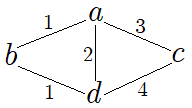
\includegraphics[width=.1875\linewidth]{images/q3b_1.png}
    \end{center}
    The minimum spanning tree of the above graph would include edges $\{ab, bd, ac\}$. The cycle $\{ac, cd, ad\}$ has $ad$ being the minimum-weight edge, which is not included in the MST.

    \pagebreak

  \item (Light-st Walk)

    My proposed algorithm has the following features:
    \begin{itemize}
      \item The algorithm takes input of (1) the adjacency list representing the graph $G$, (2) the starting vertex $s$, (3) the destination vertex $t$, and (4) the weight function $w$.
      \item The vertices and edges in this algorithm represent the vertices and edges in the given graph $G$.
      \item The edges are undirected and do not have associated values.
      \item Each vertex will have three associated values: an integer recording the minimum weight from the starting vertex, a boolean recording whether the vertex has been visited, and a place to hold the vertex's predecessor. The initial minimum weight will be set to infinite, except if the vertex is $s$, which would be set to 0.
      \item The algorithm will output a list of vertices representing the path with the minimum total weight possible to get from $s$ to $t$.
      \item The algorithm makes use of the Nonnegative Dijkstra's Algorithm with just one small modification:
        \begin{itemize}
          \item The priority queue will hold a pair: the next vertex and the current weight, just like in a regular Nonnegative Dijkstra's Algorithm. \textit{We'll use a binary min-heap as the priority queue.}
          \item The priority queue will have the pair $(s, 0)$ as a start, where $s$ is the input starting vertex.
          \item The search will go on until the queue is empty, by default. In each iteration, let's say the algorithm pops the queue and gets the pair $(x, k)$. The algorithm will skip processing $x$ if it's already visited, or otherwise it'll now mark $x$ as visited. If $x = t$, the search ends immediately, and the algorithm returns the path by going over $x$'s predecessors.
          \item Next, for each $x$'s neighbor $y$, the algorithm will add $(y, k + w(y))$ to the priority queue only if (1) $k + w(y)$ is less than $y$'s recorded minimum weight, and (2) $y$ hasn't been marked visited. If the algorithm ends up adding $y$ to the queue, it'll then record $x$ as $y$'s predecessor. The modification here is that the weight function is called on the next vertex instead of on the incident edge.
        \end{itemize}
      \item If the algorithm makes it to when the Nonnegative Dijkstra's Algorithm is over, it'll report that there isn't a path from $s$ to $t$, which might be in the form of an error.
    \end{itemize}

    Let $n$ and $m$ be the number of vertices and edges in $G$, respectively. To analyze the run-time behavior of this algorithm, let's break it down into the initialization phase and the search phase:
    \begin{itemize}
      \item The initialization phase assigns each vertex its three associated values. Since there are $n$ vertices, this part will take $O(n)$.
      \item The search phase will run in $O(n + m\log m)$, just like in a regular Nonnegative Dijkstra's Algorithm, because the only modification we did was changing how each edge weight is calculated by calling a different function (the vertex-weight function, in this case). Each vertex and each edge will still be visited the same maximum number of times just like in a Nonnegative Dijkstra's Algorithm.
    \end{itemize}

    Therefore, since the most time-consuming part of the algorithm takes $O(n + m\log m)$, the entire algorithm takes $O(n + m\log m)$.

    \pagebreak

  \item (MST Updates)

    \textbf{a.} As follows. Note that these algorithms require the adjacency list that represent the graph $G$ as an input, assuming that the user has one; if not, it should be easy to generate one in $O(|V| + |E|)$ time.

    \begin{center}
      \begin{minipage}{\linewidth}
        \renewcommand{\thealgocf}{}
        \SetArgSty{textrm}
        \begin{algorithm}[H]
          \caption{\texttt{update\_T\_on\_decrease}}
          \KwIn{\texttt{map<vertex, set<vertex>>} $A$, \texttt{set<edge>} $T$, \texttt{function} $w$, \texttt{edge} $e$}
          \KwOut{\texttt{set<edge>}}

          \If{$e \in T$}{\Return{$T$}}

          Add $e$ to $T$

          \texttt{set<edge>} $S \gets$ edges in $T$ that make a cycle, found by a Depth-First Search

          \texttt{edge} $f \gets$ edge in $S$ with the greatest weight

          Remove $f$ from $T$

          \Return{$T$}

        \end{algorithm}
      \end{minipage}
    \end{center}

    \textbf{b.}

    \begin{center}
      \begin{minipage}{\linewidth}
        \renewcommand{\thealgocf}{}
        \SetArgSty{textrm}
        \begin{algorithm}[H]
          \caption{\texttt{update\_T\_on\_increase}}
          \KwIn{\texttt{map<vertex, set<vertex>>} $A$, \texttt{set<edge>} $T$, \texttt{function} $w$, \texttt{edge} $e$}
          \KwOut{\texttt{set<edge>}}

          \If{$e \notin T$}{\Return{$T$}}

          Remove $e$ from $T$

          \texttt{set<vertex>} $R \gets$ vertices in $A$ reachable from $e[0]$ via edges in $T$, found by a Depth-First Search

          \texttt{set<edge>} $S \gets$ edges in $A$ that have exactly one endpoint in $R$

          \texttt{edge} $f \gets$ edge in $S$ with the least weight

          Add $f$ to $T$

          \Return{$T$}

        \end{algorithm}
      \end{minipage}
    \end{center}

\end{enumerate}

\end{document}
